% This Document is Copyright 2018 the authors.

% Misc. notes:
% - On model comparison figure: stuff <-60 deg more affected by gaia scan pattern, mass-loss history and stellar pop variation, disk contamination

\documentclass[12pt, modern]{aastex62}

\addtolength{\topmargin}{-0.25in}
\addtolength{\textheight}{0.50in}
\setlength{\parindent}{\baselineskip}

\newcommand{\acronym}[1]{{\small{#1}}}
\newcommand{\package}[1]{\textsl{#1}}
\newcommand{\Gaia}{\textsl{Gaia}}
\newcommand{\gaia}{\textsl{Gaia}}
\newcommand{\articlename}{\textsl{Letter}}
\newcommand{\sectionname}{Section}
\newcommand{\lcdm}{\acronym{$\Lambda$CDM}}
% \newcommand{\Tycho}{\textsl{Tycho}}
% \newcommand{\DRone}{\textsl{\acronym{DR1}}}
\newcommand{\DRtwo}{\textsl{\acronym{DR2}}}
% \newcommand{\TGAS}{\textsl{\acronym{TGAS}}}
% \newcommand{\DPAC}{{\acronym{DPAC}}}
% \newcommand{\documentname}{\textsl{Note}}
% \newcommand{\equationname}{equation}

% \newcommand{\AU}{\mathrm{A.U.}}
% \newcommand{\dd}{\mathrm{d}}
% \newcommand{\given}{\,|\,}
% \newcommand{\T}{^{\mathsf{T}}}
% \newcommand{\inv}{^{-1}}
\newcommand{\kpc}{\textrm{kpc}}
\newcommand{\msun}{\textrm{M}_\odot}

\shorttitle{dynamical evidence of a dark halo substructure}
\shortauthors{bonaca et al.}

\begin{document}\sloppy\sloppypar\raggedbottom\frenchspacing

\title{\textbf{%
Encounter of the GD-1 stellar stream with a massive perturber:\\
Dynamical evidence of a dark substructure in the Milky Way halo
}}

\correspondingauthor{Ana Bonaca}
\email{ana.bonaca@cfa.harvard.edu}

\author[0000-0002-7846-9787]{Ana Bonaca}
\affil{Harvard--Smithsonian Center for Astrophysics, 60 Garden St, Cambridge, MA 02138, USA}

\author[0000-0003-2866-9403]{David W. Hogg}
\affil{Center for Cosmology and Particle Physics, Department of Physics, New York University, 726~Broadway, New York, NY 10003, USA}
\affil{Center for Data Science, New York University, 60 Fifth Ave, New York, NY 10011, USA}
\affil{Max-Planck-Institut f\"ur Astronomie, K\"onigstuhl 17, D-69117 Heidelberg}
\affil{Flatiron Institute, 162 Fifth Ave, New York, NY 10010, USA}

\author[0000-0003-0872-7098]{Adrian~M.~Price-Whelan}
\affil{Department of Astrophysical Sciences, Princeton University, Princeton, NJ 08544, USA}

\author{Charlie Conroy}
\affil{Harvard--Smithsonian Center for Astrophysics, 60 Garden St, Cambridge, MA 02138, USA}

\begin{abstract}\noindent
% The GD-1 stellar stream is a long, thin, cold stream of stars in the Milky Way halo.
% It is sensitive to details of halo dynamics, and it has been shown to have structure that is suggestive of non-trivial gravitational interactions in its past.
We present a conceptual model for the interaction of the GD-1 stellar stream with a massive perturber that---without fine-tuning---explains many of the features of one of the stream structures, including a gap and an off-stream spur of stars.
The model involves an impulse by a fast encounter, after which the stream grows a loop of stars on different orbital energies which, at specific viewing angles, appears off the stream track.
% The model involves an impulse by a fast encounter, after which the stream grows a loop of stars that is both off the stream track, and on a set of orbits with different frequencies.
The configuration-space observations are most sensitive to a combination of mass, velocity, age, and impact parameter of the encounter, and future velocity-space observations will be sensitive to a different combination of these.
% - be more specific
Given sensible assumptions about age and velocity, the perturber must have had a mass in the range $10^6\,\rm M_\odot$ to $10^8\,\rm M_\odot$.
Orbit integrations back in time show that the stream encounter could not have been caused by any known globular cluster or dwarf galaxy, and mass and impact-parameter arguments show that it could not have been caused by a molecular cloud in the Milky Way disk.
The most plausible explanation for the gap-and-spur structure is an encounter with a dark-matter substructure, like those which are naturally predicted in this mass range in this part of the Milky Way halo in \lcdm\ cosmology.
% - leave possibility of a black hole
This observation opens up the possibility that detailed observations of streams could measure the mass spectrum of dark-matter substructures and even identify individual substructures and their orbits in the halo.

% We present a conceptual model for the interaction of GD-1, a thin Milky Way stellar stream, with a massive perturber.
% Following the encounter, the stream develops a gap at the location of the closest approach, from which emanates a loop of stream stars.
% Projected on the sky, this loop appears to extend from the stream as a narrow spur, thus reproducing the observed GD-1 morphology.
% Under the impulse approximation, we infer the length scale of impact (?) $GMT/BV = x$ from relative sizes of the gap and spur in GD-1(?).
% Encounters of GD-1 with known satellites and the Galactic disk have $GMT/BV \ll x$.
% Given how GD-1 orbits far from the Galaxy (or some better argument here), the most plausible perturber is a dark matter subhalo, which naturally populate galactic halos in the $\Lambda$CDM cosmology.
% Future kinematic maps of the perturbed region of the GD-1 stream will put constraints on the mass spectrum of dark matter subhalos in the Milky Way.

\end{abstract}

\keywords{%
cosmology:~observations
  ---
dark~matter
  ---
gravitation
  ---
stars:~kinematics~and~dynamics
  ---
Galaxy:~halo
  ---
Galaxy:~kinematics~and~dynamics
}

\section{Introduction}
\label{sec:intro}

% The clustering of dark matter (DM) on scales smaller than dwarf galaxies remains one of the most pressing unknowns in cosmology and galaxy formation \citep[for a recent review, see][]{Bullock:2017}. % TODO: also Buckley summary?
% Dark matter theories predict different minimum mass scales for clustering: In the \lcdm\ model, DM subhalos with negligible baryonic content are expected to exist in abundance with arbitrarily low masses \citep{Green:2004, Springel:2008}, while alternative models (e.g., warm DM, self-interacting DM, axion DM) have larger cut-off masses in the DM power spectrum that depend on the parameters of these models \citep{Bode:2001, Spergel:2000, Peebles:2000, Mocz:2017}.
% The detection of dark but massive substructure would therefore place strong constraints on the physics of dark matter \citep[e.g.,][]{Buckley:2017}.
% 
% Two promising prospects for detecting such structures are (1) through microlensing within and between images of strongly-lensed galaxies \citep{Vegetti:2012}, and (2) using thin stellar streams around the Milky Way \citep{Johnston:2002, Ibata:2002}.
% Thin stellar streams form from the disruption of low-mass stellar systems like globular clusters and dwarf galaxies \citep{TODO} and are thus dynamically cold structures that form through phase-mixing of tidal debris over many orbits around the Galaxy.
% Cold but dynamically old streams stretch into long, thin streams of stars that are extremely sensitive to gravitational perturbations: a gravitational encounter between a dark massive substructure and a stream leaves imprints of the encounter in the form of irregular morphological features (loops, spurs, and folds) and density variations along the stream \citep{SiegalGaskins:2008, Carlberg:2009, Yoon:2011, Ngan:2016}.
% The density variations typically evolve to form spatial under-densities --- typically referred to as ``gaps'' --- that encode information about the perturber structure, perturber orbit, and time of encounter \citep{Yoon:2011, Carlberg:2012, Carlberg:2013, Erkal:2015, Erkal:2015b}.
% 
% For low-mass perturbers ($M \lesssim 10^7~\msun$), the characteristic scale of density variations is small, $\delta\rho / \rho \sim XX\%$, and therefore requires low-contamination selection of stream stars to detect.
% For this reason, not all stellar streams within the Milky Way are equally useful for studying the presence of dark substructure: some streams lie in regions of high background density where measuring small density variations is limited by Poisson variations of the background (e.g., Hermus/Hyllus; \citealt{Grillmair:2014}), some streams cross close to the Galactic center and disk where the Galactic bar and/or molecular clouds can leave density features (e.g., Ophiuchus and Palomar 5; \citealt{Price-Whelan:2016, Pearson:2017, Amorisco:2016}), and the densest known streams are often dynamically young and very cold, so epicyclic density variations naturally arise from the formation of the stream (e.g., the Palomar 5 stream; \citealt{Kupper:2008, Kupper:2015}).
% 
% The GD-1 stream \citep{Grillmair:2006, Price-Whelan:2018} is one of the most prominent stellar streams in the Milky Way halo and has many characteristics that make it an ideal place to study the small-scale density variations that would arise from gravitational interactions with dark matter substructures.
% The stream was discovered using a matched-filter on photometry from the Sloan Digital Sky Survey (SDSS; \citealt{SDSS, TODO}).
% GD-1 is relatively close to the Sun ($d_\odot \sim 8$--$12~\textrm{kpc}$), spans at least $100^\circ$ on the sky, and is at high Galactic latitude ($20^\circ \lesssim b \lesssim 60^\circ$) where Galactic background contamination is less significant.
% Already with its discovery, hints of density variations were apparent in the surface density and map of the stream (e.g., \figurename~XX in \citealt{Grillmair:2006}).
% However, with only photometric data, the background density at the limiting magnitude of the SDSS was too high to strongly conclude about the density structure of GD-1.
% 
% Subsequent work used Megacam to obtain deeper imaging across $\approx 45^\circ$ of GD-1 (APW: check this number).
% Using a matched-filter (here with the 2-band photometry from Megacam), it became clear that the density structure of GD-1 contains prominent under-densities (gaps) and ``wiggles'' in the mean track of the stream \citep{deBoer:2018}.
% These features again suggested the tantalizing possibility that GD-1 has encountered a massive perturber.
% 
% Previous work on the GD-1 stream relied primarily on filtering photometric data to map the stream.
% Recently, using astrometric data from the second data release (\DRtwo) of the \gaia\ mission \citep{TODO}, we combined a photometric matched-filter with a kinematic matched filter to select a high-purity sample of main-sequence stars in the GD-1 stream \citep{Price-Whelan:2018}.
% The velocity of GD-1 is distinct from the foreground Galactic disk stars over most of its extent, and is much colder than the stellar halo, so the combined selection provided the highest-contrast view of a thin stellar stream in the Milky Way to date.
% With this low-contamination selection of the stream, we (1) extended the footprint of the stream to $\approx 100^\circ$, (2) confirmed the existence of at least two prominent under-densities, and (3) identified two morphological features offset from the main track of the stream (the spur and blob).
% These non-trivial features of the stream are not expected from standard models of stream formation, and therefore further motivate studying their formation.
% 
% In this \articlename, we explore the interpretation that density variations and morphological anomalies along the GD-1 stream are a result of a gravitational interaction with a dark, massive perturber.
% In \sectionname~\ref{sec:model}, we ...


\section{Encounter of GD-1 with a massive perturber}
% - present the fiducial model (fig 1)
% - comparison with the data is qualitative, data is the following (cite pwb, here is what we did in addition to select likely members)
% - define pseudo-likelihood and explain our high-level exploration of the parameter space (fig 2)
% - comment on densities of known objects in the mass-radius plane (ie compare our pdf to molecular clouds, globular clusters, central densities of dwarf galaxies, cdm subhalo predictions) (I am thinking of this as an inset to fig 2, but could be a separate figure as well)
\subsection{Features in the GD-1 stellar stream}
\label{sec:data}
GD-1 is the longest ($>100^\circ$, 10\,kpc) thin ($\sigma\approx12'$, 30\,pc) stellar stream discovered in the Galactic halo \citep{gd2006}.
Based on its width and length, GD-1 is expected to be extremely informative about the global distribution of matter in the Galaxy \citep{lux2013, bh2018}.
Indeed, dynamical modeling of GD-1 individually, and in concert with the tidal tails of the Palomar~5 globular cluster, has already revealed that the inner dark matter halo is spherical \citep{koposov2010, bowden2015, bovy2016}.
Furthermore, \citet{cg2013} used data from the Sloan Digital Sky Survey \citep[SDSS,][]{york2000} to identify gaps in stellar density along GD-1 and concluded that the number, size and depth of GD-1 gaps is consistent with $\Lambda$CDM predictions of stream perturbation by dark-matter subhalos.
However, density variations in streams at the SDSS depth can originate in part from variations in the distribution of field Milky Way stars \citep{ibata2016}, so an increase in signal-to-noise is required to ascertain the true density structure of GD-1.

Recently, \citet{pwb} used proper motions from the \gaia\ mission \citep{gdr2} and photometry from PanSTARRS \citep{ps} to confidently separate GD-1 stars from the Milky Way field stars.
This contamination-free view of GD-1 enabled the first unambiguous detection of gaps in a stellar stream, which remain evident in deeper imaging \citep{deboer2018}.
Additionally, the combined astrometric and photometric selection revealed GD-1 stars offset from the main stream track: an extended spur at $(\phi_1, \phi_2)\approx(-33^\circ,1^\circ)$ and a diffuse blob at $(\phi_1, \phi_2)\approx(-14^\circ,-1^\circ)$ in GD-1 coordinates.
Patterns imparted by the complex selection function, confusion by background galaxies, or foreground dust do not coincide with these GD-1 features; instead, they are inherent properties of the stream itself.

To highlight the complex structure of the GD-1 stream, we present the distribution of likely stream members at the top of Figure~\ref{fig:fiducial}.
As a first step in finding likely members, we followed \citet{pwb} in selecting stars consistent with an old and metal-poor population at a distance of 8\,kpc, and moving retrograde with respect to the Galactic disk, with proper motions in the GD-1 reference frame $(\mu_{\phi_1}, \mu_{\phi_2})\approx(-7,0)\;\rm mas\,yr^{-1}$.
The spatial distribution of these stars in the $\phi_2$ direction (i.e. perpendicular to the stream) is modeled as a combination of a constant background, a stream component at the location of the main stream track, and one additional Gaussian components on either side of the main stream to capture stream features beyond the main track.
We solved for the normalization, position and width of every component by exploring the parameter space with an ensemble MCMC sampler \citep{Foreman-Mackey:2013}.
We used 256 walkers that ran for a total of 1280 steps, and kept the final 256 steps to generate posterior samples in these parameters.
The above procedure is a full-stream generalization of the calculation in \citep{pwb} that quantified the fraction of stars in the additional components at the locations of the spur and the blob.
Finally, we define stream membership probability, $p_{mem}$, as the joint probability of a star belonging either to the main stream or the additional feature, and evaluate these probabilities using MCMC samples for every star.
Figure~\ref{fig:fiducial} shows stars with $p_{mem}>0.5$, with larger and darker points representing stars with a higher membership probability.

Most likely GD-1 members trace a thin stream, whose width varies between $\sigma\approx'$ and $'$.
% $\sigma\approx'$ at $\phi_1\approx-13^\circ$ to $\sigma\approx'$ at $\phi_1\approx-50^\circ$.
Stellar density along the stream is not uniform, with the most significant underdensities, or gaps, located at $\phi_1\approx-40^\circ$ and $\phi_1\approx-20^\circ$.
Additional components are above the background density in the spur region, $\phi_1\approx-35^\circ$, and the blob region, $\phi_1\approx-15^\circ$, and consistent with zero along the rest of the stream.
In the following section we present a conceptual model of GD-1 that simultaneously explains the gap in the stream and the spur extending from the stream.

\begin{figure}
\begin{center}
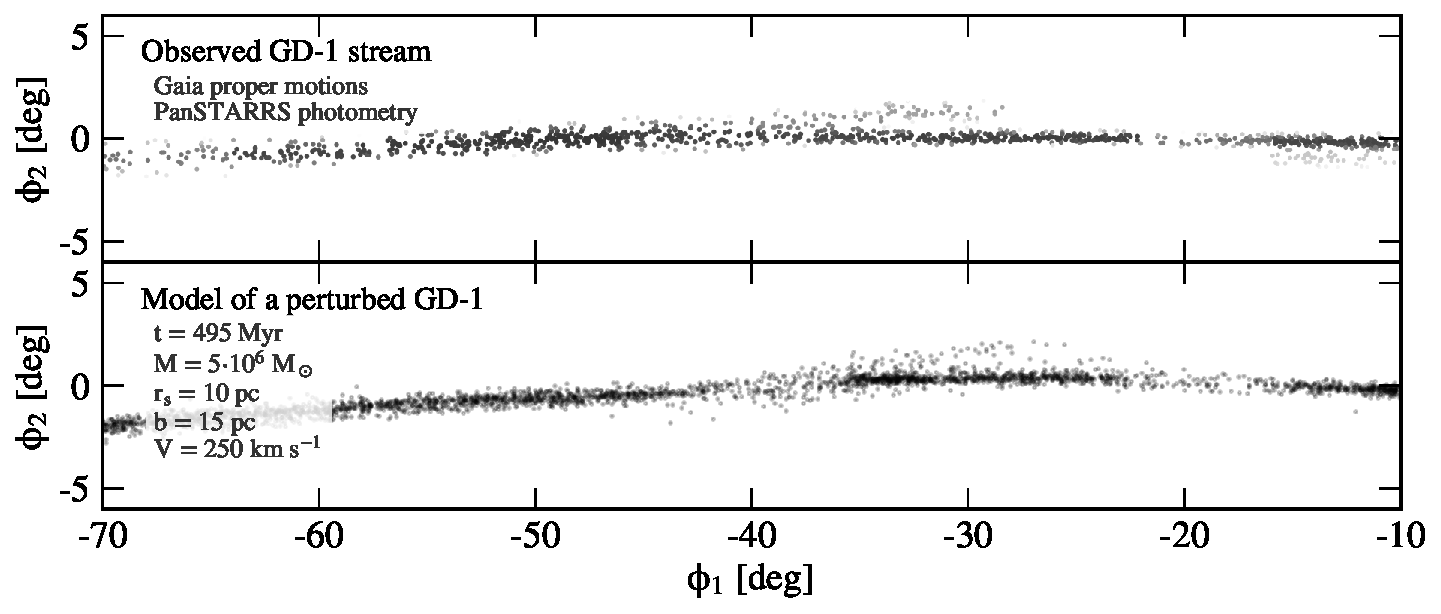
\includegraphics[width=\textwidth]{../plots/stream_encounter.png}
\end{center}
\caption{Likely members of the GD-1 stellar stream, cleanly selected using Gaia proper motions and PanSTARRS photometry, reveal an underdensity in the stream and a spur extending for $\approx10^\circ$ from this gap (top).
% The gap is $\approx8^\circ$ wide and is located at $\phi_1\approx-40^\circ$ (top right).
An idealized model of GD-1 that has been perturbed by a compact, massive object (bottom).
The orbital structure of stars closest to the passing perturber is distorted into a loop of stars that after 0.5\,Gyr appears as an underdensity coinciding with the observed gap, and extends out of the stream similar to the observed spur.
% edge-on and matches the extent of the observed spur, as well as the location and the width of the gap.
}
\label{fig:fiducial}
\end{figure}

\subsection{Perturbed model of GD-1}
\label{sec:model}
Unlike the observed gd-1, model in a smooth galaxy is also smooth \citep{pwb}, even after taking into account substructure produced by the epicyclic motions of stream stars relative to the progenitor's orbit \citep{kupper2008,kupper2010, fardal2015}.
% - streakline model \citep{fardal2015}, so it does account for substructure inherent to the process of disruption \citep{}
- can get one gap by disrupting the progenitor there
- to explain the other gap, we present a streakline model of the GD-1 stream that also had a close encounter with a dense, massive perturber

- found the orbit in potential
- follow progenitor of mass x and evaporate, until it completely disrupts x Myr before the present day
- these values were chosen to reproduce one gap morphology
- to produce the other gap, we also follow a perturber, assumed to be a Hernquist sphere of mass x and scale radius y
- the orbit of the perturber is such that it has the closest approach of x pc moving at what angle? y Myr before the present
- following the encounter, stars closest receive an energy kick, and start moving towards the location of the perturber's closest approach
- tie to gap literature
- this deforms the regular structure of a stream, which then develops a loop
- at the chosen impact geometry, this loop of stars appears edge on at the present, and looks like a spur (Figure~\ref{fig:fiducial}, bottom).

- even though the extent of the stream doesn't match, the agreement between the observed GD-1 and this model is remarkable
- in the following section we explore the range of impact parameters that still produce a good match to the observed stream

% - to uncover the origin of the gap+spur structure, we analyze a range of idealized encounters between a massive perturber and stars moving on an orbit that fits the GD-1 stream
% - the single orbit structure of the stream develops a loop after the
% - however, the stars affected by the encounter actually form a loop that extends towards the location of the closest approach (fig)
% - connect spur morphology to phases of gap growth from denis
% % - sky projections: loop can appear as a spur viewed edge-on

\subsection{Properties of the GD-1 perturber}
- for some viewing angles, a loop of stream stars formed following an encounter with a massive perturber can appear as a spur and a gap combo
- exact details depend on the following parameters: time of encounter, impact parameter, velocity, mass and size of the perturber
- to find parameters allowed by the data, we would ideally like to forward model, but generative model is hard and we don't have it
- instead, we devised a set of expert criteria that allow us to compare whether a conceptual model represents the observed structure of GD-1
- pseudo-likelihood -- ABC

\begin{figure}
\begin{center}
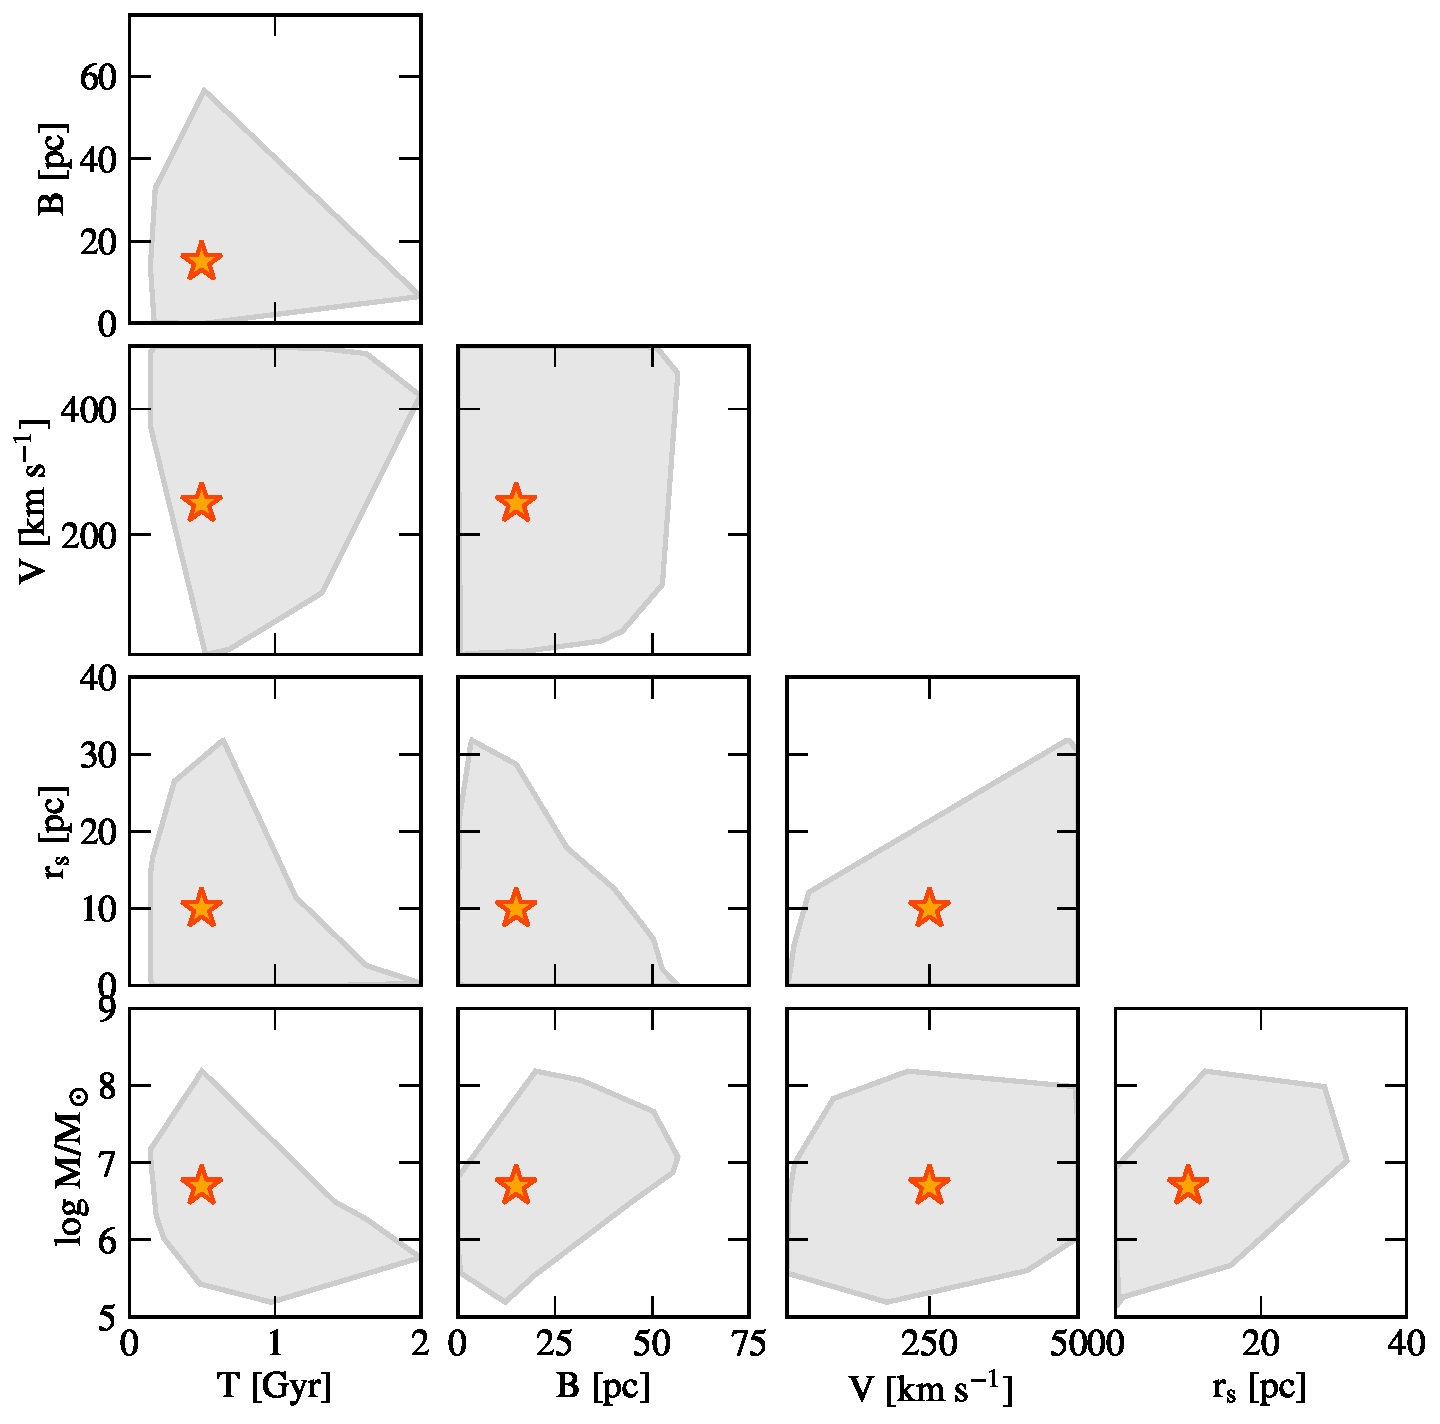
\includegraphics[width=0.8\textwidth]{corner.pdf}
\end{center}
\caption{}
\label{fig:corner}
\end{figure}

- parameter search w emcee
- comment on pdfs
- analytical argument for a young spur?

% \begin{figure}
% \begin{center}
% 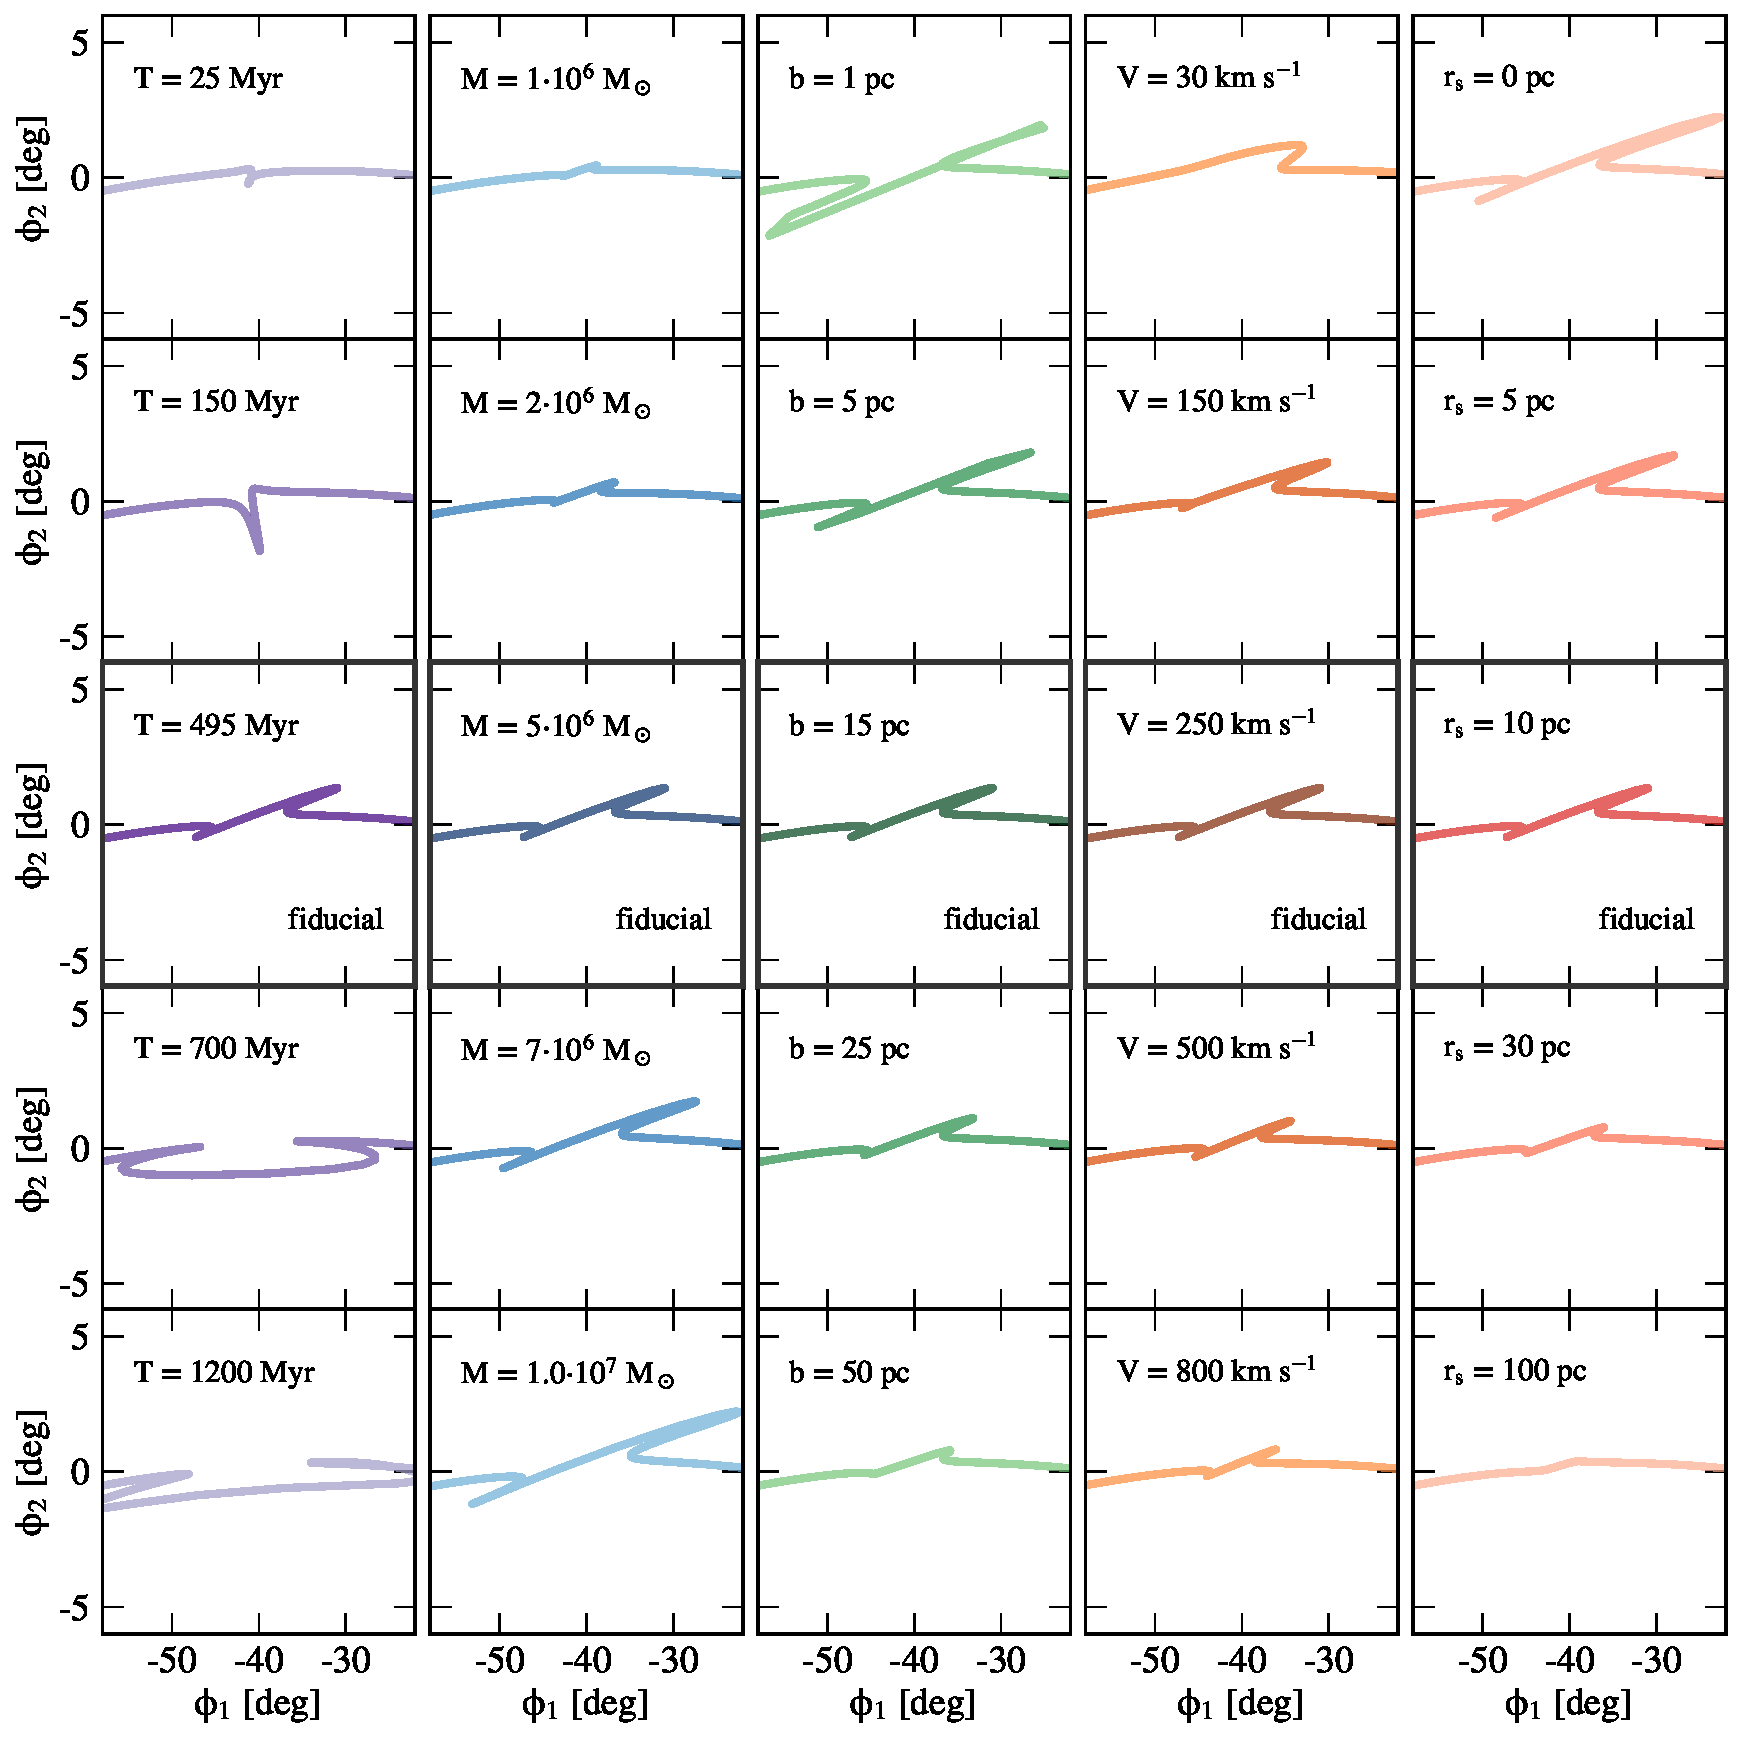
\includegraphics[width=\textwidth]{excursions.pdf}
% \end{center}
% \caption{}
% \label{fig:scalings}
% \end{figure}


\section{Origin of the GD-1 perturber}
\label{sec:origin}
- classes of objects: known satellite, unknown, disk
- integrate backwards to show that it can't be any known object.
- look at molecular cloud properties and show that they are all out.
- give some typical dm substructure numbers for the whole galaxy and for this radius range in the nearby halo.
- also something about the mass-size relationship for these dm structures.
- conclusion: dm substructure is the most plausible of the options.
- interesting point: The predictions about \lcdm\ substructure in the inner halo are controversial right now because of simulation differences. If this matters, this point should enter the abstract and modify the naturalness of the conclusion.

\begin{figure}
\begin{center}
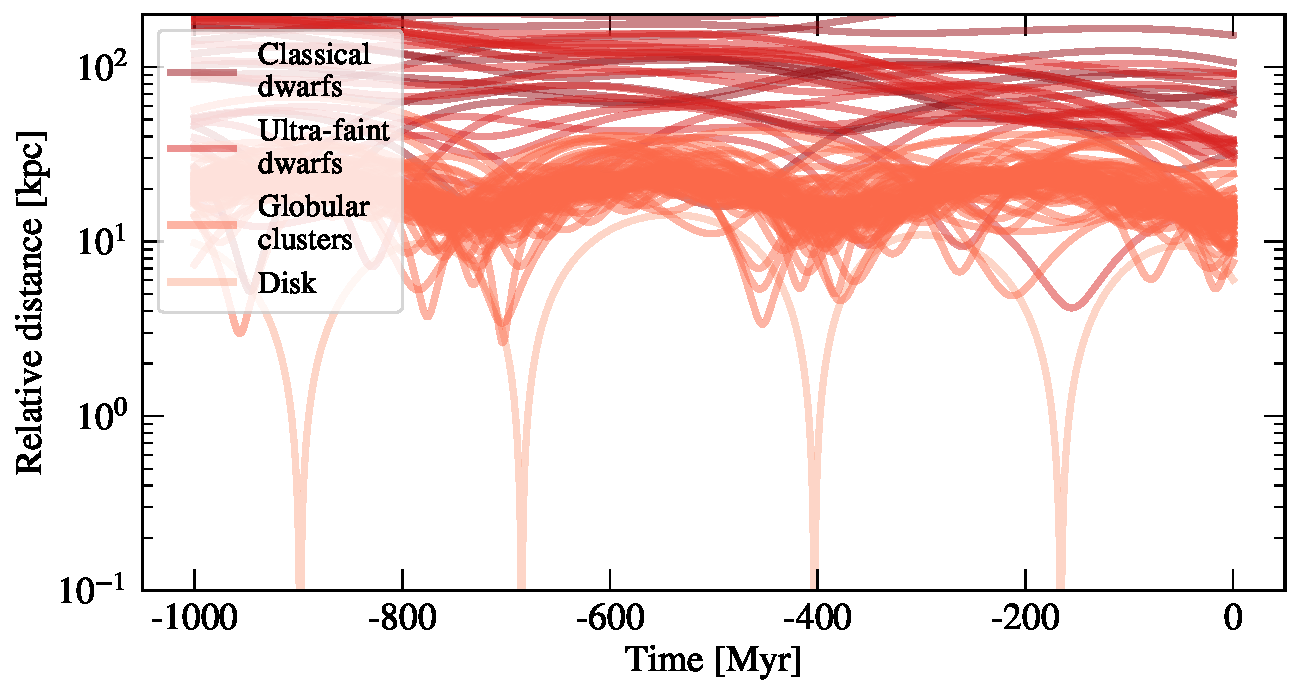
\includegraphics[width=0.8\textwidth]{satellite_distances.pdf}
\end{center}
\caption{Data from \citet{simon2018} and \citet{gdr2_satellites}.}
\label{fig:known_encounters}
\end{figure}


\section{Discussion}

% The stream perturbation models presented above show that the GD-1 stream spur and neighboring gap could plausibly be formed through a gravitational interaction between the stream and a dark, compact, massive perturber.
% By assuming this scenario for the spur and gap formation, we have compared perturbed stream models to the observed gap location and width and spur location and length, and have determined regions of encounter parameter-space that reproduce the observed morphology of the GD-1 stream.
% In this context, we have shown that the perturber would have to be a massive but compact, fast-moving object in the halo of the Milky Way.
% 
% \lcdm\ predicts that subhalos with masses between $10^6~\msun < M < 10^8~\msun$ should be abundant...
% [observed dwarfs around the Milky Way are proof of $10^7$--$10^8~\msun$]
% However, [scale radii $\sim 10$ times larger, less dense]
% 
% - compare properties to expectation from dark matter, discuss black hole possibility (but also cool!)
% 
% - Return to discussion of low-mass subhalos in simulations: baryonic sims predict far fewer subhalos, but dense ones survive? Also crazy-time: LMC replenishing subhalo population
% 
% \subsection{Alternative explanations of the spur and gap}
% % This doesn't have to remain a subsection - just putting it here for organizing
% % my thoughts!
% - When discussing alternatives: Why are they less plausible? How could we rule them out in the future, or are they ruled out now?
% 
% - SMBH: more massive than MW SMBH - where is progenitor? how did it grow?
% - GMC in disk: wrong relative velocity as GD-1 crosses midplane
% - Internal kinematics of progenitor: fine-tuned to get gap
% - Feathering from stream formation: oriented wrong way w.r.t. GD-1 orbit
% - Stream-fanning: need strong chaos for stream bifurcation. far from bar, halo likely close to spherical within orbit of GD-1
% - Luminous dwarf or globular cluster: either (1) known systems have wrong kinematic measurements, (2) unseen / unknown system, or (3) Milky Way mass distribution very different than expected. Could show difference of orbit over last 500 Myr in different potential models
% 
% 
% \section{Conclusions}
% 
% - This is huge!
% - Optimistic future of a huge network of cold streams---what might be possible?


\acknowledgements
It is a pleasure to thank Vasily Belokurov, Benedikt Diemer, Elena D'Onghia, Adrienne Erickcek, Douglas Finkbeiner, Lars Hernquist, Kathryn Johnston, Sergey Koposov, Doug Lin, Erica Nelson, Sarah Pearson, Hans-Walter Rix, and Josh Speagle + someone from CUNY for valuable discussions and input.

This project was developed in part at the 2018 \acronym{NYC} \Gaia\ \acronym{DR2} Workshop at the Center for Computational Astrophysics of the Flatiron Institute in New York City in 2018 April.

This work was performed in part at Aspen Center for Physics, which is supported by National Science Foundation grant PHY-1607611.

This work has made use of data from the European Space Agency (\acronym{ESA}) mission \Gaia\ (\url{https://www.cosmos.esa.int/gaia}), processed by the \Gaia\ Data Processing and Analysis Consortium (\acronym{DPAC}, \url{https://www.cosmos.esa.int/web/gaia/dpac/consortium}). Funding for the \acronym{DPAC} has been provided by national institutions, in particular the institutions participating in the \Gaia\ Multilateral Agreement.


\software{
\package{Astropy} \citep{astropy:2013, astropy:2018},
\package{gala} \citep{Price-Whelan:2017},
\package{emcee} \citep{Foreman-Mackey:2013},
\package{IPython} \citep{Perez:2007},
\package{matplotlib} \citep{Hunter:2007},
\package{numpy} \citep{Van-der-Walt:2011},
}

\bibliographystyle{aasjournal}
\bibliography{spur}

\end{document}
